\documentclass[bigger]{beamer}

%--------------------------------------------------
% \usepackage{pst-all} % PSTricks
% \usepackage{com.braju.pstricks} % The package that really does the hard work
% \usepackage{com.braju.graphicalmodels} % The package that really does the hard work
%-------------------------------------------------- 

\mode<presentation>{
  \usetheme{Pittsburgh}
  \usefonttheme{serif}
  \setbeamerfont{institute}{size=\normalsize}
  \setbeamerfont{section in toc}{size=\large}
  \setbeamerfont{subsection in toc}{size=\normalsize}
  \setbeamertemplate{frametitle}{%
    \vskip 12pt
    \begin{centering}
    \structure{\textbf{\insertframetitle}}\par
    \end{centering}
  }
}

\usepackage[english]{babel}
\usepackage{times}
\usepackage{algorithmic}
\usepackage{algorithm}
\usepackage{epsfig}
\usepackage{pgf}
\usepackage[absolute,overlay]{textpos}
%--------------------------------------------------
% \usepackage{mathtime}
%-------------------------------------------------- 

% Latin-1 only
\usepackage[latin1]{inputenc}
\usepackage[T1]{fontenc}
%--------------------------------------------------
% % Chinese-support
% \usepackage[nocjkbg5]{ucs}
% \usepackage[utf8x]{inputenc}
% \usepackage[C00,T1]{fontenc}
% \newcommand\tradtext[1]{\bgroup\fontencoding{C00}\fontfamily{ming}\selectfont%
% \SetUnicodeOption{cjkbg5}#1\egroup}
%-------------------------------------------------- 

\title[]{Relevance Model Revisited: With Multiple Representation}
\author[]{Ruey-Cheng Chen {\tt \scriptsize <cobain@turing.csie.ntu.edu.tw>}\\
Chiung-Min Tsai {\tt \scriptsize <cmtsai@mail.lis.ntu.edu.tw>}\\
Jieh Hsiang {\tt \scriptsize <jhsiang@ntu.edu.tw>}}
\institute{Dept. of Computer Science and Information Engineering\\
National Taiwan University, Taiwan}
\date[AIRS 2010]{AIRS 2010 (December 1, 2010)}
\subject{Information Retrieval}
%--------------------------------------------------
% \AtBeginSubsection[]
% {
%   \begin{frame}<beamer>
%     \frametitle{Outline}
%     \tableofcontents[currentsection,currentsubsection]
%   \end{frame}
% }
%-------------------------------------------------- 
%\beamerdefaultoverlayspecification{<+->}
\newcommand<>\ul[2]{\textbf{#1}\begin{itemize}#2\end{itemize} \vskip 0.5em}
\newcommand<>\ull[1]{\begin{itemize}#1\end{itemize}}
\newcommand<>\ol[2]{\textbf{#1}\begin{enumerate}#2\end{enumerate}}
\newcommand<>\oll[1]{\begin{enumerate}#1\end{enumerate}}
\newcommand<>\dl[2]{\textbf{#1}\begin{description}#2\end{description}}
\newcommand<>\f[2]{\begin{frame}{#1}#2\end{frame}}
\newcommand<>\mydef[2][]{\textbf{#1}\par#2\par}
\newcommand<>\tbl[3]{\textbf{#1}\vskip 0.5em\begin{center}\begin{tabular}{#2}#3\end{tabular}\end{center}}
\newcommand<>\fig[3]{\textbf{#1}\vskip 0.5em\begin{center}\begin{figure}\includegraphics[#2]{#3}\end{figure}\end{center}}
\newcommand<>\cols[1]{\begin{columns}#1\end{columns}}
\newcommand<>\col[2]{\begin{column}{#1}#2\end{column}}

\begin{document}

\frame{ \titlepage }

\f{Outline}{ \tableofcontents }

\section{Introduction}
\f{Homogeneous Assumption in IR}{
  
  Texts in a document is usually modeled as a set of terms, and every document
  possesses \textbf{only one} such representation

  \begin{itemize}
    \item Terms are assumed to be homogeneous \\
    (or drawn from a mixture of homogeneous sources)
    \item It leads to simple models
    \item It leaves no room for modeling heterogeneous data
  \end{itemize}
}

\f{Heterogeneous Data}{
  \begin{table}
    \centering
    \small
    \begin{tabular}{|l|l|}
      \hline
      Full-text & Long and loose textual content \\
      \hline
      Abstract & Summary of the content \\
      \hline
      Title & Short, conceptual description \\
      \hline
      Tags & Short, conceptual description (from the user side) \\
      \hline
      Metadata & Data describing the document \\
      \hline
    \end{tabular}
  \end{table}

  The data differ in scope, specificity, and semantics

  \begin{itemize}
    \item Under the homogeneous assumption, a document needs to be represented as a weighted combination
    \item Is there any other way out?
  \end{itemize}
}

\f{Idea: Layered Combination}{

  What if the model assumes \textit{multiple} document representations rather than only one?

  \begin{itemize}
    \item It is easy to incorporate heterogeneous data
    \item Retrieval can then be operated in different semantic layers
    \item Interoperation between layers is possible \\
    (and can be useful)
  \end{itemize}

  \vskip 1em
  Possible applications include

  \begin{itemize}
    \item Query expansion/refinement
    \item Facet ranking
  \end{itemize}
}

\f{Challenge: The Model}{

  To estimate the probability $\Pr(s|t)$, given that a document is indexed in
  two different vocabularies $T$ and $S$ (called the \emph{primary} and the
  \emph{secondary} term space, respectively)

  \vskip 1em
  More specifically, we want to estimate $\Pr(s|\mathbf{q})$ given the user query $\mathbf{q} \subset T$ 

  \begin{itemize}
    \item $\Pr(s|t)$ is the key to enable interactions
    \item It led us to a generalization of the relevance model \cite{lavrenko2001relevance}
  \end{itemize}
}

\section{Related Work}

\f{Related Work}{
  Our method is inspired by the recent advances on language modeling
  \begin{itemize}
    \item Relevance model \cite{lavrenko2001relevance}
    \item Smoothing in language modeling \cite{zhai2001language}
    \item Bayesian language model \cite{zaragorza2003bayesian}
  \end{itemize}

  \vskip 1em
  Similar attempts toward facet ranking were made in the area of expert finding
  \begin{itemize}
    \item Inverse entity-frequency \cite{amitay2008finding}
    \item language-model-based approach \cite{balog2009language} 
  \end{itemize}
}

\f{Roadmap}{

  Our approach differs in:
  \begin{itemize}
    \item The presence of a secondary document representation
    \item The way document relevance is modeled 
    \item The way prior belief is supported
  \end{itemize}

  \vskip 1em
  Where do we go from here?
  \begin{itemize}
    \item We introduce an adapation of the relevance model \cite{lavrenko2001relevance}
    (to cases where two representations are appropriate)
    \item We derive the model using Bayesian generative approach
    \item Two applications are introduced to evaluate our work 
  \end{itemize}
}

\section{Model}
\subsection{The Generative Framework}

\begin{frame}[fragile]
  \frametitle{The Generative Framework}
  \begin{figure}
    \centering
    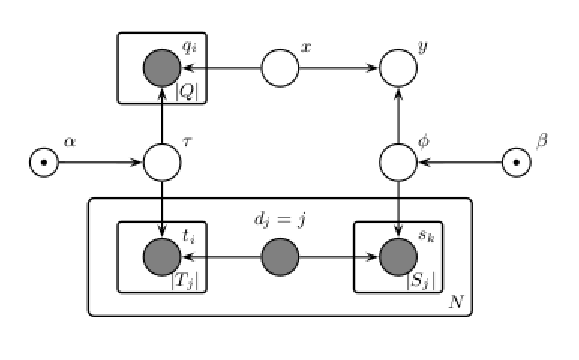
\includegraphics[width=8cm]{model}
  \end{figure}

  \begin{itemize}

    \only<1>{ \item Document $d_j$ is associated with two sets of terms $T_j$
    and $S_j$  }
    
    \only<2>{ \item Elements in $T_j$ and $S_j$ are drawn from two multinomials
    $\tau^{(j)}$ and $\phi^{(j)}$, respectively  }
    
    \only<3>{ \item Two Dirichlets priors $\{\alpha_i; i \in [1, |T|]\}$ and
    $\{\beta_k; k \in [1, |S|]\}$ are assumed }

    \only<4>{ \item Some unknown document has generated $\mathbf{q}$ and $y$
    (an unknown secondary term)}

  \end{itemize}

\end{frame}

\f{Generative Process}{
  For each document $d_j$:
  \begin{enumerate}
    \item $\tau^{(j)} \sim \textrm{Dirichlet}(\alpha_i; i \in [1, |T|])$
    \item $\phi^{(j)} \sim \textrm{Dirichlet}(\beta_k; i \in [1, |S|])$
    \item For $i \in \{ 1, \ldots, |T_j| \}$, $t_i \sim \textrm{Mult}(\tau^{(j)})$ 
    \item For $k \in \{ 1, \ldots, |S_j| \}$, $s_k \sim \textrm{Mult}(\phi^{(j)})$ 
  \end{enumerate}

  \vskip 1em
  \textbf{Goal}: Find $y^*$ by using the predictive distribution 
  \begin{equation} y^* = \arg\max_{y \in S} \Pr(y|\mathbf{q},
  \mathbf{t}, \mathbf{d}, \mathbf{s}) \label{eq:forward} \end{equation} 
  \begin{itemize}
    \item $\mathbf{t}$, $\mathbf{s}$, $\mathbf{d}$, $\mathbf{q}$: all the observed primary/secondary terms, documents, and query
  \end{itemize}
}

\subsection{Inference}

\f{Exact Inference}{
  \begin{eqnarray}
    && \Pr(y|\mathbf{q}, \mathbf{t}, \mathbf{d}, \mathbf{s})
    = \sum_{x \in [1, N]} \Pr(y|x, \mathbf{q}, \mathbf{t}, \mathbf{d}, \mathbf{s}) \Pr(x|\mathbf{q}, \mathbf{t}, \mathbf{d}, \mathbf{s}) \nonumber\\
    &\propto& \sum_{x \in [1, N]} \left\{ \int \Pr(y|x, \phi^{(x)}) \Pr(\phi^{(x)}|d_x, \mathbf{s_x}) \mathrm{d}\phi^{(x)} \right. \nonumber\\
    && \left. \int \Pr(\mathbf{q}| x, \tau^{(x)}) \Pr(\tau^{(x)}|d_x, \mathbf{t_x})\mathrm{d}\tau^{(x)} \Pr(x) \right\} \nonumber\\
    &=& \alert{\sum_{x \in [1, N]} \frac{\beta_y + c_{y,x}}{\sum_k \beta_k + c_{k,x}} \frac{\mathcal{B}(\{\alpha_i + c_{i,x} + c_{i,q} \})}{\mathcal{B}(\{\alpha_i + c_{i,x} \})} \Pr(x)} \label{eq:forward-solution}
  \end{eqnarray}
  \begin{itemize}
    \item $\mathcal{B}(\cdot)$ is the multinomial beta
    function defined by $\mathcal{B}(a_1, \ldots, a_n) = (\prod_i
    \Gamma(a_i)) / \Gamma(\sum_i a_i)$
  \end{itemize}
}

\subsection{Hyperparameters and the Index Structure}

\f{Hyperparameters}{
  \ul{Prior distributions}{
    \item Prior represents our belief on the distribution of the model parameters
    \item General form: $(\beta_1, \beta_2, \ldots, \beta_{|S|})$
  }
  \par

  \ul{Uniform prior}{ \item $(c, c, \ldots, c)$ \item We let $\beta_k = c$ for
  each $k \in [1, |S|]$ and $c$ denote some constant }

  \ul{Smoothed-Dirichlet}{
    \item $(\mu \Pr(s_1|C), \mu \Pr(s_2|C), \ldots, \mu \Pr(s_{|S|}|C))$ 
    \item $\Pr(s_k|C)$ denotes the probability of generating term $s_k$ (in the secondary
term domain) from the collection by viewing the entire collection as one language model
    \item $\mu$ represents some constant.
    \item Widely-used as a smoothing method in the language modeling applications for information retrieval \cite{zhai2004study}
  }
}

\f{Index Structure}{
  \ul{Integration with the language model}{
    \item One interesting feature of our model is the seamless integration
    with the language-model-based retrieval method
    \item It comes from
    the fact we could further simplify Equations~\eqref{eq:forward-solution} by
    assigning $\alpha$ as a smoothed-Dirichlet prior and $\Pr(x)$ as a uniform
    prior
    \item When $\alpha_i = \mu \Pr(t_i|C)$, it can be shown that: \[
    \frac{\mathcal{B}(\{\alpha_i + c_{i,x} + c_{i,q} \})}{\mathcal{B}(\{\alpha_i +
    c_{i,x} \})} \propto {\rm L}_{\rm LM}(\mathbf{q}|d), \] where ${\rm L}_{\rm
    LM}(\mathbf{q}|d)$ denotes the query likelihood score in the language model
    with Dirichlet smoothing scheme
    
    \item In this case, the model scores becomes:
    \begin{eqnarray}
      \Pr(y|\mathbf{q}, \mathbf{t}, \mathbf{d}, \mathbf{s}) &\propto& 
      \alert{\sum_{x \in [1, N]} \frac{\beta_y + c_{y,x}}{\sum_k \beta_k + c_{k,x}}
      {\rm L}_{\rm LM}(\mathbf{q}|x)}
    \end{eqnarray} 
  }
}


\section{Experimental Results}
\subsection{Query Refinement Using the Secondary Representation}

\f{Query Refinement Using the Secondary Representation}{
  \ul{Idea}{
    \item Make an initial retrieval run
    \item Use the retrieved result to populate the refined model
    \item Re-submit the model as a new query
  }
  \par
  \ul{Why employing two-stage retrieval?}{
    \item $\Pr(y|\mathbf{q}, \mathbf{t}, \mathbf{d}, \mathbf{s})$ can be seen as a refined query model
    \item This technique was proposed in Lavrenko's work
    \item The new model is refined in the secondary representation
    \item The benefit of such a two-stage setup: \ull{
      \item The first run is done in general language (good for recall)
      \item The second run is done in specific language (good for precision)
    }
  }
}

\f{Query Refinement Using the Secondary Representation}{
  \ul{Facilatating the second-run retrieval}{
    \item The refined model is a probability distribution
    \item For each $s_k$, we calculated its \emph{expectation} $E(s_k|\mathbf{q}, \mathbf{t}, \mathbf{d}, \mathbf{s})$
    \item The expectation can be seen as the number of occurrence for $s_k$
    \item The resulting language model is: \[
      x^{*} = \arg\max_x \prod_k \Pr(s_k|x)^{E(s_k|\mathbf{q}, \mathbf{t}, \mathbf{d}, \mathbf{s})}
    \]
    \item This simple technique reduces to KL-divergence retrieval framework \cite{zhai2001language}
  }
}

\f{Evaluation}{
  \ul{Setup}{
    \item Task: Chinese-to-Chinese monolingual document retrieval
    \item The benchmark is available as part of NTCIR-4 Test Collection CLIR Task
    \item 381,681 newswire articles and 59 test topics were involved
    \item We used only title queries in the experiment 
    \item Primary representation: CJK-character bigrams + English word unigrams
    \item Secondary representation: High-discriminative CJK-character bigrams \ull{
      \item I.e., top-500,000 CJK-character bigrams ranked by tf-idf scores
      \item The minimum support for each bigram was 5
      \item The number (500,000) was determined through experimentation
    }
  }
}

\f{Evaluation}{
  \ul{Baseline methods}{
    \item We used the Lemur toolkit to build up strong baselines
    \item Participating runs include tf-idf, okapi, and indri (a language-model variant)
    \item Query refinement/expansion for each run: \ull{
      \item tf-idf: pseudo relevance-feedback
      \item okapi: pseudo relevance-feedback
      \item indri: adapted relevance model
    }
    \item The number of feedback documents: 20
    \item The number of feedback terms: 100
    \item Our refined model was truncated (preserving only top-100's)
    \item Performance was measured in terms of mean average-precision and precision-at-5
  }
}

\f{Evaluation Result}{
  \begin{table}[ht!]
    \scriptsize
    \centering
    \begin{tabular}{lllll}
      Method & MAP (+\%) & P@5 (+\%) & MAP (+\%) & P@5 (+\%) \\
      \hline
      {\tt tfidf} & 0.181 & 0.264 & 0.213 & 0.335 \\
      {\tt tfidf} + PRF & 0.217 (+19.9\%) & 0.295 (+11.7\%) & 0.264 (+23.9\%) & 0.383 (+14.3\%) \\
      {\tt okapi} & 0.185 & 0.278 & 0.223 & 0.356 \\
      {\tt okapi} + PRF & 0.224$^{**}$ (+21.1\%) & 0.315 (+13.3\%) & 0.270$^{**}$ (+21.1\%) & 0.400 (+12.4\%) \\
      \hline
      {\tt indri} & 0.174 & 0.258 & 0.216 & 0.346 \\
      {\tt indri} + Relevance & 0.180 (+3.4\%) & 0.271 (+5.3\%) & 0.222 (+2.8\%) & 0.342 (-1.2\%) \\
      {\tt lm} & 0.170 & 0.251 & 0.209 & 0.322 \\
      {\tt lm} + Refinement & 0.207$^*$ (+21.8\%) & 0.302 (+20.3\%) & 0.261$^*$ (+24.9\%) & 0.369 (+14.6\%) \\
      \\
    \end{tabular}

    \caption{The result for the query refinement task.  Retrieval methods listed in the
    upper-half are tfidf-based, while those in the lower-half are
    language-model-based.  The overall top-performer is indicated with two
    asterisks in the superscript, while the best run in the language-modeling
    side is indicated with one asterisk.}
    \label{t:query-modeling}
  \end{table}
}

\subsection{Retrieving Query-Relevant Facets}

\f{Retrieving Query-Relevant Facets}{
  \ul{Faceted search as a two-phase extension of the ordinary retrieval}{
    \item See \cite{hearst2002finding,yee2003faceted,roy2008minimum} for detail about faceted search
    \item One populates a set of documents by submitting the query
    \item One discovers facets by exploiting the associations between facets and documents 
    \item How do we present the facets?
  }
  \par
  \ul{Count-based presentation schemes}{
    \item Facets are sorted in descending order of the number of counts
    \item It is easy to implement (one more pass through the forward index)
    \item It treats all the facet count as equally importatnt \ull{
      \item e.g., A facet count in document \#1 is as good as in document \#100
    }
    \item Critics \#1: It disregards the notion of relevance
    \item Critics \#2: Users can be mislead when consulting the results to guide the subsequence exploratory search
  }
}

\f{Retrieval Query-Relevant Facets}{
  \ul{Idea}{
    \item Encode facets in the secondary representations of the corresponding associated documents
    \item Run the proposed model
  }
  \par
  \ul{Why using the secondary representation?}{
    \item This task is relevant to (but not equivalent to) expert finding 
    \item Use $\Pr(y|\mathbf{q}, \mathbf{t}, \mathbf{d}, \mathbf{s})$ to sort the facets
    \item Consider this method as a relevance-weighted version of the count-based approach
    \item It is efficient: fast as ad-hoc retrieval (with a little overhead forwarding scores)
  }
}

\f{Evaluation}{
  \ul{Setup}{
    \item Task: Retrieving relevant facets on Tan-Hsin Corpus
    \item The test data comprises 15,314 historical documents, each with person name facets
    \item 105 query topics are collected from the query logs 
    \item 28 topics were randomly selected and used in the experiment
    \item Relevance judgment was manually made for all the top 100 facets returned by the baseline retreiver
  }
  \par
  \ul{Methods}{
    \item \texttt{baseline}: The count-based scheme
    \item \texttt{uniform-prior}: The proposed method, using uniform prior for $\beta$
    \item \texttt{smoothed-prior}: The proposed method, using Dirichlet-smoothed prior for $\beta$
  }
}

\f{Evaluation Result}{
  \begin{table}[ht!]
    \centering
    \begin{tabular}{llll}
      Method & & MAP & P@10 \\
      \hline
      {\tt baseline} & & 0.2996 & 0.3857 \\
      {\tt uniform-prior} & $\beta = 0$ & 0.5775 & 0.6179\\
      & $\beta = 1$ & 0.5899$^*$ & 0.6464$^*$ \\
      & $\beta = 10$ & 0.5877 & 0.6464$^*$ \\
      {\tt smoothed-prior} & $\mu = 0.01$ & 0.5781 & 0.6179 \\
      & $\mu = 1$ & 0.5782 & 0.6214 \\
      & $\mu = 100$ & 0.4956 & 0.5429 \\
      \\
    \end{tabular}
    \caption{The performance results for all the test runs.  The top-performer is indicated by an asterisk in the superscript.}
    \label{t:performance}
  \end{table}
}

\section{Discussion and Concluding Remarks}
\f{Discussion and Concluding Remarks}{
  \ul{Our proposed framework...}{
    \item Enables the use of a secondary document representation in language modeling
    \item Offers interoperability between two different term domains
    \item Exploits the index structure to achieve high efficiency
  }

  \ul{Evaluation results}{
    \item Two applications were introduced in this work
    \item In the first task, the model beaten the relevance model baseline by 17.6\% (rigid) and 22.7\% (relax) in 
    MAP \ull{ 
      \item It achieved comparable performance as {\tt tfidf} with pseudo-relevance feedback
      \item The model alone improved the MAP of the regular language modeling run by 21.8\% (rigid) and 24.9\% (relax)
    }
    \item In the second application, the baseline performance was improved by
    roughly 100\% in MAP.  
  }
}

\section<presentation>*{\appendixname}

\begin{frame}[allowframebreaks]
  \frametitle{References}
  \small
  \bibliography{slides}
  \bibliographystyle{alpha}
\end{frame}

\f{Inference: Step by Step}{
  \mydef[Inducing the first term in the summation]{
    \begin{eqnarray}
      \Pr(y|\mathbf{q}, \mathbf{t}, \mathbf{d}, \mathbf{s}) &=& \sum_{x \in
      [1, N]} \alert{\Pr(y|x, \mathbf{q}, \mathbf{t}, \mathbf{d}, \mathbf{s})}
      \Pr(x|\mathbf{q}, \mathbf{t}, \mathbf{d}, \mathbf{s}) \nonumber\\
      && \nonumber\\
      \Pr(y|x, \mathbf{q}, \mathbf{t}, \mathbf{d}, \mathbf{s})
      &=& \int \Pr(y, \phi^{(x)}|x, \mathbf{q}, \mathbf{t}, \mathbf{d}, \mathbf{s}) \mathrm{d}\phi^{(x)} \nonumber\\
      &=& \int \Pr(y|\phi^{(x)}, x, \mathbf{q}, \mathbf{t}, \mathbf{d}, \mathbf{s}) 
      \Pr(\phi^{(x)}|x, \mathbf{q}, \mathbf{t}, \mathbf{d}, \mathbf{s}) \mathrm{d}\phi^{(x)} \nonumber\\
      &=& \int \Pr(y|\phi^{(x)}, x) \Pr(\phi^{(x)}|d_x, \mathbf{s}_x) \mathrm{d}\phi^{(x)} \label{eq:first}
    \end{eqnarray}
  }
}

\f{Inference: Step by Step}{
  \mydef[Inducing the second term in the summation]{
    \begin{eqnarray}
      \Pr(y|\mathbf{q}, \mathbf{t}, \mathbf{d}, \mathbf{s}) &=& \sum_{x \in
      [1, N]} \Pr(y|x, \mathbf{q}, \mathbf{t}, \mathbf{d}, \mathbf{s})
      \alert{\Pr(x|\mathbf{q}, \mathbf{t}, \mathbf{d}, \mathbf{s})} \nonumber\\
      && \nonumber\\
      \Pr(x|\mathbf{q}, \mathbf{t}, \mathbf{d}, \mathbf{s})
      &=& \frac{\Pr(\mathbf{q}|x, \mathbf{t}, \mathbf{d}, \mathbf{s}) \Pr(x|\mathbf{t}, \mathbf{d}, \mathbf{s})}
      {\Pr(\mathbf{q}|\mathbf{t}, \mathbf{d}, \mathbf{s})} \nonumber\\
      &\propto& \Pr(\mathbf{q}|x, \mathbf{t}, \mathbf{d}, \mathbf{s}) \Pr(x|\mathbf{t}, \mathbf{d}, \mathbf{s}) \nonumber\\
      &=& \left( \int \Pr(\mathbf{q}, \tau^{(x)}|x, \mathbf{t}, \mathbf{d}, \mathbf{s}) \mathrm{d}\tau^{(x)} \right) 
      \Pr(x|\mathbf{t}, \mathbf{d}, \mathbf{s}) \nonumber\\
      &=& \left( \int \Pr(\mathbf{q}|\tau^{(x)}, x, \mathbf{t}, \mathbf{d}, \mathbf{s}) 
      \Pr(\tau^{(x)}|x, \mathbf{t}, \mathbf{d}, \mathbf{s}) \mathrm{d}\tau^{(x)} \right) 
      \Pr(x|\mathbf{t}, \mathbf{d}, \mathbf{s}) \nonumber\\
      &=& \int \Pr(\mathbf{q}|\tau^{(x)}, x) \Pr(\tau^{(x)}|d_x, \mathbf{t}_x) \mathrm{d}\tau^{(x)} \Pr(x) \label{eq:second}
    \end{eqnarray}
  }
}

\f{Inference: Step by Step}{
  \ul{Conjugate priors}{
    \item In Bayesian theory, the prior $\Pr(\theta)$ and posterior $\Pr(\theta|x)$
    are called conjugate distributions, if the posterior are in the same family as the prior
    \item Usually, it can be viewed as updating the prior belief on
    $\theta$ after observing a sequence of outcome $x$.
    \item Conjugate prior is an algebraically ``syntactic sugar'' to simplify inference
    \item Fast fact: Dirichlets are conjugate to multinomials \ull{
      \item $\Pr(\phi^{(x)}|x, y, d_x, \mathbf{s}_x) \sim \mathrm{Dirichlet}(\{\beta_k + c_{k,x}; \forall k\})$
      \item $\Pr(\tau^{(x)}|x, \mathbf{q}, d_x, \mathbf{t}_x) \sim \mathrm{Dirichlet}(\{\alpha_i + c_{i,x} + c_{i,q}; \forall i\})$
    }
  }
  \par
  \ul{Care for going into details?}{
    \item Detailed derivation is too terrifying/boring to be presented here
    \item Check out Gelman et al. for good reference on Bayesian statistics
  }
}

\f{Inference: Revisited}{
  \mydef[Integrating out the prior]{
    \begin{eqnarray}
    \int \Pr(y|x, \phi^{(x)}) \Pr(\phi^{(x)}|d_x, \mathbf{s_x}) \mathrm{d}\phi^{(x)} 
    &=& \frac{\beta_y + c_{y,x}}{\sum_k \beta_k + c_{k,x}} \\
    \int \Pr(\mathbf{q}| x, \tau^{(x)}) \Pr(\tau^{(x)}|d_x, \mathbf{t_x})\mathrm{d}\tau^{(x)} 
    &=& \frac{\mathcal{B}(\{\alpha_i + c_{i,x} + c_{i,q} \})}{\mathcal{B}(\{\alpha_i + c_{i,x} \})} 
    \end{eqnarray}
  }
  \par
  \mydef[Voila!]{
    \begin{eqnarray}
      \Pr(y|\mathbf{q}, \mathbf{t}, \mathbf{d}, \mathbf{s}) 
      &=& \sum_{x \in [1, N]} \Pr(y|x, \mathbf{q}, \mathbf{t}, \mathbf{d}, \mathbf{s}) \Pr(x|\mathbf{q}, \mathbf{t}, \mathbf{d}, \mathbf{s}) \nonumber\\
      &\propto& \alert{\sum_{x \in [1, N]} \frac{\beta_y + c_{y,x}}{\sum_k \beta_k + c_{k,x}} \frac{\mathcal{B}(\{\alpha_i + c_{i,x} + c_{i,q} \})}{\mathcal{B}(\{\alpha_i + c_{i,x} \})} \Pr(x)}
    \end{eqnarray}
  }
}

\frame{
  \begin{center}
    \Huge{Thanks for your attention!}
    \par
    Any Question?
  \end{center}
}

\end{document}
